%!TEX program = XeLaTeX
%!TEX encoding = UTF-8 Unicode

%%%%%%%%%%%%%%%%%%%% book.tex %%%%%%%%%%%%%%%%%%%%%%%%%%%%%
%
% sample root file for the chapters of your "monograph"
%
% Use this file as a template for your own input.
%
%%%%%%%%%%%%%%%% Springer-Verlag %%%%%%%%%%%%%%%%%%%%%%%%%%


\documentclass[graybox,envcountchap,sectrefs]{svmono}

% choose options for [] as required from the list
% in the Reference Guide

\usepackage{mathptmx}
\usepackage{helvet}
\usepackage{courier}
%
\usepackage{type1cm}

\usepackage{makeidx}         % allows index generation
\usepackage{graphicx}        % standard LaTeX graphics tool
                             % when including figure files
\usepackage{multicol}        % used for the two-column index
\usepackage[bottom]{footmisc}% places footnotes at page bottom
\usepackage[numbers]{natbib}

% support Chinese
%\usepackage{CTex}
%\usepackage{ctex}
\usepackage[UTF8]{ctex}

\usepackage{amsmath,bm}
\usepackage{amssymb}
\usepackage{color}
\usepackage{graphicx}
%\usepackage[unicode]{hyperref}
\usepackage{xcolor}
\usepackage{float}
\usepackage{indentfirst}
\usepackage{enumerate}
%\usepackage{epstopdf}
%\usepackage{titlesec}
\usepackage{mathrsfs}
\usepackage[ruled,linesnumbered]{algorithm2e}
\usepackage{epsfig,tabularx,amssymb,amsmath,subfigure,multirow,graphicx}
%\usepackage{fontspec}
\usepackage{diagbox}
\usepackage{longtable}
\usepackage{hyperref}

% see the list of further useful packages
% in the Reference Guide

\makeindex             % used for the subject index
                       % please use the style svind.ist with
                       % your makeindex program

%%%%%%%%%%%%%%%%%%%%%%%%%%%%%%%%%%%%%%%%%%%%%%%%%%%%%%%%%%%%%%%%%%%%%

\begin{document}

%\author{CSLT}
\title{自然语言处理与生物识别}
\subtitle{Natural Language Processing and Biometric Identification}
\maketitle


\frontmatter%%%%%%%%%%%%%%%%%%%%%%%%%%%%%%%%%%%%%%%%%%%%%%%%%%%%%%

%\include{dedic}
%\include{foreword}
%\include{preface}
%\include{acknow}

\tableofcontents

%\include{acronym}

\mainmatter%%%%%%%%%%%%%%%%%%%%%%%%%%%%%%%%%%%%%%%%%%%%%%%%%%%%%%%
%%%%%%%%%%%%%%%%%%%%% chapter.tex %%%%%%%%%%%%%%%%%%%%%%%%%%%%%%%%%
%
% sample chapter
%
% Use this file as a template for your own input.
%
%%%%%%%%%%%%%%%%%%%%%%%% Springer-Verlag %%%%%%%%%%%%%%%%%%%%%%%%%%
%\motto{Use the template \emph{chapter.tex} to style the various elements of your chapter content.}
\chapter{NLP发展现状与应用领域}
\label{basic} % Always give a unique label
% use \chaptermark{}
% to alter or adjust the chapter heading in the running head

\section{定义简介}
自然语言处理(Natural Language Processing,简称NLP),属于计算机科学与语言学的交叉学科,所以又称计算语言学;它是用计算机来理解、处理、运用人类语言的学科。人类通过自然语言进行沟通协作,可以说如果没有语言人类的智能将无从谈起,它是人类区别于动物的重要标志。也可以说,只有当计算机具备了准确的自然语言的理解处理能力时,才算真正实现了人工智能。
\begin{itemize}
\item 研究内容:NLP研究内容主要包括词法分析、句法分析、语义分析、篇章理解、机器翻译等。
\item 应用场景:NLP广泛应用信息系统方方面面。例如:手写体识别、光学符号识别、语音识别、语音合成、信息检索、机器翻译、对话系统等。
\item 关联学科:NLP紧密相关的研究领域包括机器学习、数据挖掘、知识图谱等;紧密相关的学科包括信息论、语言学、计算机科学等。
\end{itemize}

NLP研究范围涉及自然语言的形态学、语法学、语义学和语用学等几个层次。
\begin{itemize}
\item 形态学(morphology):研究词的内部结构,包括屈折变化和构词法两个部分。
\item 语法学(syntax):研究句子结构成分之间的相互关系、句子序列的组成规则。
\item 语义学(semantics):研究各级语言单位(词素、词组、句子、段落、片等)的意义,以及与语音、语法、语境的关系等等,其重点在探明符号与其所指对象之间的关系。
\item 语用学(pragmatics):研究在不同上下文下的语句应用,以及上下文对语句理解所产生的影响。大概来说,语用学研究范围问题是很广,重点在于研究包括直指、会话隐含、预设、语言行为、话语结构等。
\end{itemize}

NLP面临的两大难题是歧义消解、未知语言现象。
\begin{itemize}
\item 歧义消解:在自然语言的词法、句法、语义等各个层次中存在大量的歧义现象。比如“什么是一个词”,这就是NLP面临的一个难题。因为不同的人对词语粒度、标准有不同的理解。再比如,语言中存在大量一词多义的现象,在上下文语境中如何准确找到对应的词义,这些都是NLP研究面临的实实在在的难题。
\item 未知语言现象:未知语言现象主要由两个方面的原因导致。第一点,人类语言一直处于不断演化过程中,同一个语言表达,在新的时空环境下,可能已经不再是以前的含义;而且,由于信息网络的发达,人们构造、传播新语言现象的能力大大增强,比如互联网上每天都在涌现新的语言词汇。第二点,在NLP研究中,由于整理收录能力、知识表达能力等现实因素的制约,实际中并没有一种可以准确、全面表达人类语言知识工程或工具。
\end{itemize}

\section{发展历史}
NLP发展历史中存在两种不同的的研究方法:基于规则的理性主义;基于统计的经验主义。它们对语言的不同理解,体现了它们不同的哲学思想。
\begin{itemize}
\item 理性主义:认为自然语言是由语言规则来产生和描述的;因此他们相信,只要能够用适当的形式将人类语言规则表示出来,就能够理解人类语言。
\item 经验主义:认为语言知识可以从语言数据中获取,只要建立有效的统计模型就可以理解语言;因此他们相信,如果有足够多语言数据用于统计,就能够理解人类语言。
\end{itemize}

NLP发展历史可以总结为5个时期:
\begin{enumerate}
\item 经验主义萌芽时期:时间大约到20世纪50年代。这个时期NLP或多或少具有经验主义色彩。例如,1913年马尔科夫提出马尔科夫模型\cite{markov1913example}的时候,就曾经计算过长诗中元音与辅音出现的频度概率;再比如,1948年,香农把离散马尔科夫的概率模型应用于语言自动机\cite{shannon1948mathematical}的时候,也曾统计过英语字母的频率。

\item 经验主义低谷时期:时间从1956年~20世纪90年代。1956年,乔姆斯基首先提出使用有限状态机来刻画自然语言\cite{chomsky1956three}。具体来说,就是使用数学的代数、集合论为基础核心,将各种语言现象统一抽象为代数、集合上的运算规则。形式语言理论影响深远,在此后很长一段时期,很多学者逐步完善并扩展了形式语言理论。这段时期,NLP领域的研究方法几乎完全被理性主义主导,经验主义被打入谷底。

\item 经验主义复苏时期:时间从20世纪50年代末到90年代初期。虽然这期间,例行理性主义占据主流,但是有学者已经开始思考引入基于语料库的统计方法到NLP研究中;这其中的代表是1967年诞生的联机语料库Brown Corpus\cite{kuvcera1967computational}。另外,和NLP紧密相关的机器学习方法得到了较大的发展;比如这段时期,诞生了贝叶斯模型、最大熵\cite{jaynes1957information}、维特比算法\cite{viterbi1967error}、隐马尔可夫模型\cite{stratonovich1965conditional}等等,NLP研究有了更多理论工具可供使用。

\item 经验主义爆发时期:时间20世纪90年代中期~2010年左右。时间处于20世纪90年代前期,此刻经验主义已经处于全面复苏的前夜。一方面,由于机器学习领域诞生了很多新理论和方法,推动了NLP快速发展;另一方面,计算机的存储容量、计算能力已经极大提升,使得很多计算量偏大的机器学习方法逐渐实用。受益于这两方面,经验主义终于开始全面复苏,迎来了一个前所未有的黄金时期。20世纪90年代以后,以语料库和统计学习为基础,基于机器学习的词法分析、句法分析、机器翻译、语音识别等研究不断涌现。

\item 经验主义现代时期:时间从2003年左右至今。这段时期,经验主义再上高峰,具有更加鲜明的特色,神经网络、深度学习的是目前NLP研究的关键词。Ruder在博文\cite{ruder2018review}在中总结了这段时期里NLP的研究趋势,其中以神经语言模型(Nerual Language Model,NLM)、多任务学习(Multi-task Learning)、词嵌入(Word Embedding)、Seq2Seq(Sequence To Sequence Model)模型、注意力(Attention)机制、基于记忆的网络(Memory-based Networks)、预训练语言模型(Pretrained Language Models)等这个时期重要的里程碑。

\end{enumerate}

\section{应用领域}
自然语言处理研究的内容非常广泛,应用范围也非常广泛,如下举例一些常见的应用场景:
\begin{itemize}
\item 机器翻译:利用计算机实现自然语言(英语、汉语等)之间的自动翻译。
\item 自动摘要:利用计算机自动地从原始文档中提取全面准确地反映该文档中心内容的简单连贯的短文。
\item 文本分类:在预定义分类体系下,根据文本的特征,将给定文本于一个或多个类别相关联的过程。
\item 情感分类:根据文本所表达的含义和情感将文本划分为褒扬或者贬义的两种或几种类型,是对作者倾向性、观点、态度的划分,因此也称倾向性分析。
\item 信息抽取:从非结构化或半结构的自然语言文本中提取出于某个主题相关的实体、关系。事件等事实信息,并且形成结构化信息输出。
\item 信息检索:用户输入一个表述需求信息的查询字段,系统回复一个包含所需要信息的文档列表。其核心技术在于索引构建和相关性计算。
\item 问答系统:接受用户自然语言形式描述的问题,从大量异构数据中查找或者推断用户问题答案的信息检索系统。
\end{itemize}



%%%%%%%%%%%%%%%%%%%%% chapter.tex %%%%%%%%%%%%%%%%%%%%%%%%%%%%%%%%%
%
% sample chapter
%
% Use this file as a template for your own input.
%
%%%%%%%%%%%%%%%%%%%%%%%% Springer-Verlag %%%%%%%%%%%%%%%%%%%%%%%%%%
%\motto{Use the template \emph{chapter.tex} to style the various elements of your chapter content.}
\chapter{语言模型与主题模型}
\label{lm}

本章简单介绍自然语言处理中的语言模型和主题模型的概念及其应用。


\section{语言模型}

语言模型(Language Model)用于计算语言序列$w_1, w_2, \cdots, w_n$的概率,数学表示为$P(w_1, w_2, ..., w_n)$,它是对语句的概率分布的建模。
其最直接的应用就是判断一句话来自于人生成的语句的概率,例如在我们自然语言中,句子``我去吃饭''相比于``吃饭去我''的出现的概率更高,因此$P($``我去吃饭''$) > P($``吃饭去我''$)$。讲到这里,最直接的一个问题就是,如何计算$P(w_1, w_2, ..., w_n)$呢?我们下面介绍一种最基本的语言模型:n-gram语言模型。

n-gram语言模型是一种最基础的语言模型。根据链式法则(Chain Rule),公式$P(w_1, w_2, ..., w_n)$可以得到:
\begin{equation} \nonumber
\label{equ:ab}
\begin{aligned}
P(w_1, w_2, \cdots, w_n)=P(w_1)P(w_2|w_1)\cdots P(w_n|w_1,\cdots,w_{n-1})
\end{aligned}
\end{equation}
其中的每一项$P(w_i|w_1,\cdots,w_{i-1})$,可以用以下公式来估计,即:
\begin{equation} \nonumber
\label{equ:ab}
\begin{aligned}
P(w_i|w_1,\cdots,w_{i-1}) = \frac{C(w_1,\cdots, w_{i-1}, w_i) }{C(w_1,\cdots,w_{i-1})}
\end{aligned}
\end{equation}
其中,$C(\cdot)$表示该序列在训练语料中出现的次数。但是,当序列长度很长时候,计算$P(w_i|w_1,\cdots,w_{i-1})$比较困难,一种常见的处理方式是引入马尔可夫假设(Markov Assumption),即假设当前词出现的概率只依赖于前$n-1$个词,也就是:
\begin{equation} \nonumber
\label{equ:ab}
\begin{aligned}
P(w_i|w_1,\cdots,w_{i-1}) = P(w_i|w_{i-n+1},\cdots,w_{i-1})
\end{aligned}
\end{equation}
根据$n$取值的不同,我们可以得到不同的n-gram语言模型:
\begin{itemize}
    \item Unigram: $P(w_1, \cdots, w_{i-n})=\prod_{i=1}^{n} P(w_i)$
	\item Bigram: $P(w_1, \cdots, w_{i-n})=\prod_{i=1}^{n} P(w_i|w_{i-1})$
	\item Trigram: $P(w_1, \cdots, w_{i-n})=\prod_{i=1}^{n} P(w_i|w_{i-1},w_{i-2})$
\end{itemize}

在计算n-gram时候,一个很重要的问题就是测试集中出现了训练集中未出现过的词而导致语言模型计算出的概率为零,我们称这些词为未登录词(OOV)。平滑(Smoothing)技术就是为了缓解这类问题,常见的平滑技术有:拉普拉斯平滑(Laplace Smoothing),、古德图灵法(good-turing)、线性减值法(Linear Discounting)等,感兴趣的读者可以深入阅读相关论文。

\begin{figure}[h!]
	\begin{center}
		\includegraphics[width=0.9\textwidth]{img/chapter_lm/asr-pipeline2.png}
		\caption{语音音识别基本流程}
		\label{pic:asr}
	\end{center}
\end{figure}

自动语音识别(Automatic Speech Recognition,ASR)是一种将人的语音转换为文本的技术,它是目前很多互联网产品如语音助手,语音搜索引擎等中必不可少的一部分。
图~\ref{pic:asr}给出了常见的语音识别系统的基本工作流程。其中基本可以分为以下几个模块:
\begin{itemize}
    \item 数据预处理: 典型的预处理包含静音处理(Voice Activity Detection,VAD)等,用于去除其中的静音片段。
	\item 特征提取:将声音转换成包含声音信息的多维向量,常见的有MFCC等。
	\item 声学模型:主要是通过语音数据训练得到,其输出是音素等信息。
	\item 词典:字/词和音素之间的对应关系。
	\item 语言模型:也就是上文提到的语言模型部分,主要用于评估字或者词序列的概率。
\end{itemize}

\noindent 语音系统首先将语音信号做特征提取工作,转化成诸如MFCC等特征来表示,然后使用语言模型和声学模型来解码,解码过程会产生很多候选(Candidates),最终最优的候选会被输出成为最终的结果。语言模型是其中很重要的一部分,它用于从根据语言统计规律评估声学模型给出的句子序列候选的概率,决定了最终输出的结果。


\section{主题模型}

主题模型 (Topic Models) 是近些年来非常重要的一项技术,它被广泛应用于工业和学术界。在主题模型中,我们一般用$d$来表示要分析的文档,例如一篇文章或者一个网页等,而一个文档$d$通常由一系列词$(w_1, w_2, ..., w_n)$组成, 其中$w_n$ 是文档中的第$n$个词。多份文档共同构成了我们要分析的语料集,我们用$\mathcal{D}$来表示,$\mathcal{D}=(d_1, d_2, ..., d_m)$ 组成,其中$d_m$ 是语料库中的第$m$个文档。主题一般用$z$来表示,它由一些词组成,同时也有该词在这个主题下的概率。主题模型泛指由一类可以从语料库中抽取主题并利用这些主题表示文档的模型,常见的主题模型有PLSA,LDA,以及各种LDA的变种,例如SentenceLDA等。在熟悉了这些基本概念之后,我们通过一种常见的主题模型Latent Diriclet Allocation (LDA)来认识主题模型。

\begin{figure}[htb]
	\begin{center}
		\includegraphics[width=0.8\textwidth]{img/chapter_lm/lda.png}
		\caption{LDA图模型}
		\label{pic:lda}
	\end{center}
\end{figure}


2003年Blei等人在《Latent Dirichlet Allocation》~\cite{blei2003latent} 一文中提出了LDA 模型。
如图\ref{pic:lda}所示,其中空心节点表示隐藏变量,实心变量表示客观测变量,整个模型具有K 个主题,M个文档和N个词。
LDA将文档的主题分布$P(z|d)$看做随机变量$\theta$,并且假设$\theta$从一个狄利克雷先验中产生。
同时,由于训练数据之外的文档对应的主题分布$\theta$可以从上述狄利克雷分布中产生,训练数据之外的文档的$\theta$可以更自然地进行计算。读者可以使用常见的开源主题模型工具如LightLDA\cite{yuan2015lightlda}、Familia\cite{jiang2018familia}来尝试训练LDA模型。近年来,出现了各种对主题模型的扩展工作,例如联邦学习场景下的主题模型\cite{jiang2019federated}工作等。





%\begin{figure}[htb]
%	\begin{center}
%		\includegraphics[width=0.8\textwidth]{img/chapter_lm/lma2.png}
%		\caption{语言模型适配}
%		\label{pic:lma}
%	\end{center}
%\end{figure}

%语音识别系统中一个常见的问题就是,我们训练语言模型的语料和它实际线上应用的语料之间存在不一致,这种情况下,除了重新训练模型,有一种代价更小的方法就是语言模型适配(Language Model Adaptation)。
%语言模型适配指的是用实际应用的语料相关的信息,对语言模型做适配。图~\ref{pic:lma}给出了其常见的工作流程,采用预先训练好的主题模型,我们对语音识别系统第一遍识别出来的词网格
%(Word Lattice)做主题推断,可以发现其语义级别的内容,同时它也可以作为一个unigram的语言模型$P_{LDA}(w|\theta_d)=\sum_{k \in K} \varphi_{kw} \theta_{dk}$,对之前的n-gram语言模型就行适配:
%\begin{equation}
%\begin{aligned}
%P_{d}(w|C) = \lambda P_{LDA}(w|\theta_d) + (1-\lambda) P_{n-gram \ LM}(w|C)
%\end{aligned}
%\label{eq:hb_model}
%\end{equation}
%其中$C$代表当前词$w$的上下文,$\lambda$是一个权重参数,$P_{n-gram\ LM}(w|C)$是基础的ngram语言模型给出来的评估分数。这个新适配过的语言模型,可以用于语音识别系统,重新解码出新的词网格以及最终的结果。


\chapter{词法,语法与语义分析}
\label{basic} % Always give a unique label
% use \chaptermark{}
% to alter or adjust the chapter heading in the running head

\section{词法分析}
\subsection{问题定义}
词法分析是自然语言处理的第一步,是做NLP深层次分析的先决条件。词法分析的核心是,将自然语言解析为词序列,并判断每个词的词性、专名信息,为后续分析做好准备。总的来说,在中文这种孤立语中,词法分析主要由分词、词性标注、命名实体识别3个子任务组成。

\begin{itemize}
\item 自动分词(Word Segmentation):是将连续的自然语言文本,切分成具有语义合理性和完整性的词汇序列的过程。
\item 词性标注(Part-of-Speech Tagging):是指为自然语言文本中的每个词汇赋予一个词性的过程。
\item 命名实体识别(Named Entity Recognition,也称专名识别):是指识别自然语言文本中具有特定意义的实体,主要包括人名、地名、机构名、时间等。
\end{itemize}

\begin{figure}[h!]
\centering
\includegraphics[scale=0.5]{img/chapter_nlp/lexical_example.png}
\caption{词法分析示例}
\label{fig:lexical_example}
\end{figure}

如图\ref{fig:lexical_example}所示,将输入句子切分成词序列,然后给每个词汇标记出名词、动词、介词等词性;并且识别出“2003年10月15日”是时间,识别“杨利伟”是人名等。

因为词法分析的自动分词、词性标注、专名识别本质上是类似的,所以它们的发展历史方也是类似的。总结起来,都大致经历词典匹配、机器学习、深度学习这3个发展阶段。

\subsection{实现方案}

\subsubsection{词典匹配}
\noindent
基于词典匹配的实现步骤:

\begin{enumerate}
\item 词典构建:根据具体任务的语言学知识构建词典。如果是自动分词,则收录常见词条;如果是词性标注、专名识别,则收录当前常见词条,并记录对应词性、专名属性的概率分布。
\item 词典匹配:扫描输入序列,得到任务的DAG图表示。图中每条边都是词典词条,每种首尾贯通的路径都是一种候选结果。只要求解DAG图的最优路径,则可以得到输入序列的结果。
\item 歧义消解:由于候选之间存在歧义,所以基于词典匹配之上,需要加入一些启发式规则以解决歧义问题。常用规则主要包含最大前向匹配(Forward Maximum Matching,FMM)、最大后向匹配(Backward Maximum Matching,BMM)、最少切分、双向最大匹配、长片段优先等策略\cite{wong1996chinese}\cite{weichun2013research}。
\end{enumerate}

很长一段时间内研究者都在对基于词典匹配方法进行优化,比如采用TRIE索引树\cite{yang2012enhanced}、哈希索引\cite{li2003new}等、AC自动机\cite{ngword}等结构方便快速查找。

基于词典匹配的优缺点:
\begin{itemize}
\item 优点:实现简单、运行速度快
\item 缺点:面临词典收录更新困难、未登录词难处理;同时由于消除歧义策略过于简单,通常效果不甚理想。
\end{itemize}

\subsubsection{机器学习}
\noindent
基于机器学习的实现步骤:

\begin{enumerate}
\item 转换为序列标注问题:通过定义标注空间,将任务转换为序列标注问题。以分词为例:常用BIES表示每个字在词中的位置。B表示词的开始(Begin), I表示词的中间(Inside), E表示词的结尾(End),S表示单字词(Singleton)。这种标注空间的划分在词性标注和专名识别任务上也很常用,比如专名识别中常用BIO标签集。
\item 求解序列标注问题:传统序列标注模型主要包括隐马尔科夫模型(Hidden Markov Model,HMM)\cite{zhang2003chinese}\cite{kupiec1992robust}\cite{yu2006chinese}\cite{morwal2012named}、最大熵马尔科夫模型(Maximum Entropy Markov Model,MEMM)\cite{mccallum2000maximum}\cite{ratnaparkhi1996maximum}\cite{borthwick1999maximum}、条件随机场(Conditional Random Field,CRF)\cite{zhao2006improved}\cite{constant2011mwu}\cite{ekbal2008named}、结构化感知机(Structural Perception Machine)\cite{zhang2007chinese}\cite{zhang2008joint}等浅层模型。这些浅层模型的区别主要在于如何对待输入字序列和标签序列之间的概率,训练目标是最大联合概率似然、最大条件概率似然,还是最小化风险等。
\end{enumerate}

总结来说:传统序列标注模型中,CRF是集大成者。相比于HMM,CRF去除了输出独立性要求,对于整个序列内部的信息和外部观测信息都可以有效利用,可以更加有效建模上下文。相比于MEMM,CRF通过全局归一化(global normalization),避免了MEMM locally normalized导致的label bias缺陷。

以自动分词任务为例,则其序列标注任务定义为:
定义标签集为$L=\{B, I, E, S\}$,给定输入文本序列$X=\{x_{1}, x_{2}, ..., x_{n}\}$,目标是求解最优标注序列$Y^{*}=\{y^{*}_{1}, y^{*}_{2}, ..., y^{*}_{n}\}$:

\[y^{*}=\mathop{\arg\max}\limits_{Y \in L^{n}} p(\bm{Y}|\bm{X})\]

预测时,使用维特比算法求解最优标注序列$Y^{*}$;训练时,使用最大化条件似然来训练模型,其中,$f_{i}$为人工定义的特征函数:

\[p_{w}(Y|X)=\frac{1}{Z_{w}(x)}\exp(\sum_{i} w_{i} f_{i}(y_{i}, y_{i-1}, x))\]

\[Z_{w}(x)=\sum\limits_{y \in Y}\exp(\sum_{i} w_{i} f_{i}(y_{i}, y_{i-1}, x))\]

\noindent
基于机器学习的优缺点:
\begin{itemize}
\item 优点:通过人工设计的特征工程,充分地挖掘了序列的上下文信息。模型的歧义消解胜过词典匹配的方法;同时具有很强的泛化能力,能够很好地处理未登录词问题。
\item 缺点:特征工程不经需要耗费大量人力,而且需要大量语言学知识,设计和寻找有效特征存在较高门槛;另外,这些浅层模型,通常使用离散的binary特征,无法表达复杂先验,比如没法利用词向量。
\end{itemize}

\subsubsection{深度学习}
随着大数据、神经网络、深度学习的快速发展,很多研究提出利用前馈神经网络来解决词法分析\cite{collobert2011natural}\cite{zheng2013deep}任务。总的来说,与前面基于机器学习的方法类似,也是把词法分析任务作为序列标注问题进行求解,只是把人工设计特征函数,改成了使用多层前馈神经网络进行自动特征抽取。

后续有很多研究,深度学习框架基础上,对前馈神经网络进行改进,进一步探索了卷积神经网络\cite{wu2019neural}、循环神经网络\cite{chen2015long}、递归神经网络\cite{chen2015gated}等复杂结构对词法分析任务的影响。

另外,传统的词法分析通常会把分词、词性标注、命名实体识别当成pipeline形式的进行处理,这样容易导致错误传播问题。比如,如果分词任务出现错误,将会导致后续词性标注、专名识别、句法分析、语义分析出现错误。所以在学术界也有很多联合建模\cite{zhang2008joint}\cite{hatori2012incremental}\cite{shao2017character}的工作,通过多个任务联合学习,以期望避免错误传播。联合建模的优点:各个子任务可以充分共享有用信息,通常可以取得比单任务更好的结果。联合建模的缺点:解码空间变大,搜索的复杂度提高,需要更有效的搜索剪枝机制在降低搜索复杂度的同时,尽量保持搜索结果的质量。

值得一提的是,2018年诞生了ELMO\cite{peters2018deep}、GPT\cite{radford2018improving}、BERT\cite{devlin2018bert}这3个杰出代表。它们通过将语言模型嵌入作为特征,使用目标任务数对语言模型对进行微调,使得众多NLP任务都获得了大幅度提升,这其中就包括了自动分词、词性标注、专名识别。

总结起来,基于深度学习方法的优点是通过深度神经网络自动学习多层特征抽象,避免了复杂的特征工程;模型的歧义消解、泛化能力通常都很好。只是,深度学习模型需要训练充分,通常对数据量、计算量都有较高的要求。

\subsection{应用案例}
通常NLP中深层次的语法语义分析通常都是以词作为基本单位,所以词法分析都是这些深层次分析的基础和先决条件。词法分析作为自然语言处理的第一步,是下游所有分析任务的基础。这些下游应用小句法分析、语义分析,大到对话系统、文本分类、自动摘要、机器翻译\cite{chang2008optimizing}、信息检索、搜索引擎、语音合成等等。几乎只要有利用到自然语言处理技术的地方,词法分析都是不可或缺的基础技术。

比如在搜索引擎中,用户输入查询,系统回复包含所需要信息的文档列表。其核心技术在于索引构建和相关性计算。索引构建:需要对文档进行,分词、词性标注、专名识别,为所有文档建立倒排索引。相关性计算:需要对query进行词法分析,然后以词为粒度计算query和文档的相似度。


\section{语法分析}
\subsection{问题定义}
短语结构语法(Constituency Structure Grammar)和依存关系语法(Dependency Grammar)是现在常见的两种语法关系。短语结构语法又叫上下文无关文法 (Context-Free Grammars,CFGs),它从一个特殊的初始符号出发,不断的应用一些产生式规则,从而生成出一个字串的集合(如句子)。产生式规则指定了某些符号组合如何被另外一些符号组合替换。
它呈现一个树分类关系,句法根据一定的规则进行转换分析。每一个词的转换都是需要按照设定的树值规则进行目的性的转换。

依存语法(从属关系语法) 是由法国的语言家Lucien Tesnière提出的\cite{tesniere1959elements},
它将句子各个词语之前的搭配关系描述成预先定义好的依存关系。它基于一个基本假设:句法结构本质上包含词和词之间的依存(修饰)关系。一个依存关系连接两个词,分别是核心词(head)和依存词(dependent)。依存关系可以细分为不同的类型,表示两个词之间的具体句法关系。比如主语依赖于谓语(SBV),宾语也依赖于谓语(VOB)以及定语依赖于名词性短语(ATT)等。依存句法认为“谓语”中的动词是一个句子的中心,其他成分与动词直接或间接地产生联系。

除了以上介绍的两种句法体系外,国内外都开展了对句法分析的研究。不论是国外的链语法(Link Grammar) 、组合范畴语法(Combinatory categorial grammar,CCG)等,还是国内黄曾阳教授提出的HNC理论(Hierarchical Network of Concept)\cite{黄曾阳:12}都是目前行业内常用的语法,只是由于设定区域的不同,所以使用有一定的局限性。

短语结构分析的语法集是由固定的语法集组成,较为固定和呆板,依存语法则更加的自由。另外依存语法树标注简单且parser准确率更高,再加之通用依存数据集(Universal Dependencies Treebanks)的发展,依存语法分析受到专家学者普遍的青睐,得到越来越多的应用。这里也将着重介绍依存语法分析。

\begin{figure}[h]
\centering
\includegraphics[scale=0.3]{img/chapter_nlp/parser_example.png}
\caption{LTP依存句法分析样例}
\label{fig:parserexample}
\end{figure}
例如,从上述例子中我们可以看到,句子的核心谓词为“强调”,主语(SBV)是“他”,强调的宾语(VOB)是“紧迫性”,“紧迫性”的修饰语(ATT)是“武汉疫情控制”。


\subsection{实现方案}
依存句法分析方法主要可以分为两种,一种是基于图的方法(Graph Based),一种是基于转移(Transition Based)的方法。基于图的方法先建立句子中所有词语的全连接图,然后求图中的最大生成树。 两种方法中更主流的算法是基于转换的依存句法分析,基于转移的方法将依存树的构成过程建模为一个动作序列,将依存分析问题转化为寻找最优动作序列的问题。基于转移的解析过程是线性的,动作步骤随句子长度线性增长,而基于图的方法需要在全图上做搜索,所以时间复杂度上基于转移的方法会有优势。但是基于转移的方法在解析的每一步都只是利用局部信息,会导致错误传播,性能比基于图的略差。

近几年,分别出现了针对这两种不同方法的神经网络模型。比如基于图的\cite{dozat2016deep, ji2019graph, ma2017neural},直接用神经网络来预测每两个词之间存在依存关系的概率,得到一个全连接图,图上每个边代表了节点 $a$ 指向节点 $b$ 的概率, 然后使用MST等方法来来将图转换为一棵树。概率的计算可以简单的使用节点$a$和节点$b$的embedding向量做向量运算,也可以使用复杂的多层GNN网络迭代更新。 基于转移的如 \cite{fernandez2019left, kiperwasser2016simple, ma2018stack},通过两个LSTM 来分别建模stack状态、buffer状态,使用第三个LSTM网络或者Pointer网络来建模动作序列。 
\begin{figure}[h]
\centering
\includegraphics[scale=0.3]{img/chapter_nlp/parser_nn.png}
\caption{基于转移的算法Stack-Pointer Networks for Dependency Parsing 网络结构图}
\label{fig:parser_nn}
\end{figure}


\subsection{应用案例}
依存语法分析在信息检索,评价抽取和情感分析等NLP任务上都有很多应用。比如“谢霆锋的儿子是谁”和
“谢霆锋是谁的儿子” 两句话如果不使用依存语法分析,很有可能就返回了一样的结果。依存句法分析能够更直接地通过语法结构的规则约束筛选出可能正确结果,提升相应任务的准确性。又比如“深圳大学非常漂亮,学生都很聪明”,这里 “漂亮” 形容的是 “深圳大学”, “聪明”形容的是“学生”,通过依存句法分析,就可以抽取出对应的搭配。再比如“我家音响声音很大”和“我家洗衣机声音很大”,两者在情感上前者是正评价,后者是负评价,需要使用依存句法分析来识别“声音很大”的修饰对象。

常用的中文依存句法分析的工具有复旦大学fnlp\footnote{\url{https://github.com/FudanNLP/fnlp}},斯坦福大学 Stanford CoreNLP\footnote{\url{https://stanfordnlp.github.io/CoreNLP/}}, Hanlp\footnote{\url{https://github.com/hankcs/HanLP}}和哈工大 LTP\footnote{\url{https://github.com/HIT-SCIR/ltp}}。





\section{语义分析}
在自然语言处理领域,语义分析涉及在某种程度上理解单词、短语、句子或文档的意义。传统狭义语义分析主要包括语义消歧(word sense disambiguation)\cite{ yarowsky1995unsupervised}和语义角色标注(semantic role labeling)\cite{ carreras2005introduction, bjorkelund2009multilingual}。语义消歧指在给定文本上下文中确定多义词语的含义。
%例如,“他买了一台新苹果,用来修图更方便了”中,苹果一次指代苹果电脑,而非水果。
语义角色标注是给词语和短语标注其在上下文文本中的含义的过程,典型标注标签包括主体、意图、结果等。
% 如图\ref{fig:semantic_role_label}。语义角色标注是面向任务型对话系统中核心组件自然语言解析模块的基础技术之一。

% \begin{figure}[h]
% \centering
% \includegraphics[scale=1]{img/chapter_nlp/guang_analysis_1.png}
% \caption{语义角色标注示例}
% \label{fig:semantic_role_label}
% \end{figure}

随着深度神经网络在自然语言处理领域的应用和研究,基于神经网络的语义分析得到了越来越多的应用和发展,并成为了驱动神经机器翻译\cite{ bahdanau2014neural, luong2015effective}、阅读理解\cite{ hermann2015teaching}、对话系统\cite{ serban2016building, chen2017survey}的最基础和核心的技术。基于神经网络的语义分析广义上可分为语义表示和语义匹配。其中语义表示任务将词语和短语镶嵌到高维向量空间中,称作词向量,作为CNN\cite{ lecun1995convolutional}、RNN\cite{ hochreiter1997long}和Transformer\cite{ vaswani2017attention}等模型的底层输入,根据任务需要,可以灵活的实现文本分类\cite{ joulin2016bag, zhang2015character}、机器翻译、阅读理解、对话系统、文本摘要\cite{ tan2017abstractive, yao2017recent}等自然语言处理任务,逐步替代或部分替代了传统以ngram one-hot向量作为底层表示的方法。语义匹配任务更多关注句子和篇章层级的语义的相似性,例如,寻找给定语料库中与查询语句语义层面最相似的句子。语义匹配任务在信息抽取、对话系统、问答系统都有广泛的应用。

\subsection{语义表示}
语义表示中词向量的概念可以追溯到Bengio的著作\cite{ bengio2003neural}。作者在文中提出了一种基于神经网络的语言模型,创新的提出将每一个词表示成一个高维的向量,而后使用神经网络计算给定上文词语后,下一个词出现的概率分布,最大化训练语料出现的概率。
%训练语料是单词序列$w_1, \cdots, w_t, w_t \in V$,其中$V$是全体单词的集合。语言模型的目标是找到一个模型$f(w_t, \cdots, w_{t-n+1}) = P(w_t|w_1 ^ {t-1})$,即在给定前$t-1$个词的情况下,对第$t$个词的概率分布建模。Bengio提出把词表示成实数向量,$C(i) \in \mathbb{R}^m$,即每一个词对应一个维度为$m$的实数向量,映射$C$可以用一个$|V| \times m$的实数矩阵表示。在第二步中,作者提出使用神经网络$g$来建模给定前缀序列下一个词的概率。模型结构如图~\ref{fig:neural_language_model}。
其中,将词表示成高维实数向量的方法是词向量以及一系列神经网络在自然语言处理应用的开端。通常,我们会设计一个仅与文本结构或上下文相关的(无监督)任务作为目标,拟合训练数据,得到词向量表示。在Bengio之后,Word2Vec\cite{ mikolov2013distributed}, Glove\cite{ pennington2014glove}, ELMo\cite{ peters2018deep}等一系列词向量方法出现并逐渐成为自然语言处理的标准工具。
语义表示不仅限于词的层面,广义的语义表示在现代基于神经网络的自然语言处理中应用广泛。例如,神经机器翻译通常采用编码器译码器(Encoder-Decoder)\cite{ sutskever2014sequence}结构,其中编码器的输出可以看做是翻译模型对输入文本的语义表示,译码器基于该表示,生成目标语言的文本。再如,闲聊型对话系统中,需要针对聊天的上文给出合适的回答。闲聊对话系统可以分为生成式对话系统(Generation-based)\cite{ shang2015neural}和选择式对话系统(Selection-based)\cite{ chen2017survey}。选择式对话系统依赖语义匹配方法。典型的生成式闲聊对话系统也采用编码器译码器结构,其中编码器的输出是对聊天上文的总结性表示,可以认为是广义上的聊天上文的语义表示,用于在译码器中生成合适的回答语句。此外,随着自然语言处理预训练模型的发展,Bert\cite{devlin2018bert},GPT-2\cite{ radford2019language},MASS\cite{ song2019mass}等预训练模型(Pretrained models)在阅读理解等任务上大放异彩。这些模型可以看做是多个联合任务共享底层语义表示的学习,通常使用与文本结构相关的目标作为训练目标,设计神经网络结构表示文本。在应用时,这些预训练获得的表示仅需在少量标注数据上进行优化,即可获得优秀的子任务模型。通常,编码器和预训练模型采用CNN、RNN、Transformer等结构处理文本序列,在CNN和RNN中通常还会使用注意力(Attention)机制,得到文本片段的语义表示。
%
% \begin{figure}[h!]
% \centering
% \includegraphics[scale=1]{img/chapter_nlp/guang_represent_1.png}
% \caption{一种使用词向量的神经语言模型结构}
% \label{fig:neural_language_model}
% \end{figure}

\subsection{语义匹配}
语义匹配任务在语义表示的基础上,对文本片段之间的相似度或相关度给出量化指标,语义越相似的片段匹配分数越高。语义匹配可大致分为基于表示的匹配(representation-based matching)\cite{ feng2015applying}和基于交互的匹配(interaction-based matching)\cite{ zhou2018multi, luspatio}。
基于表示的匹配方法注重对表示层的构建。常见的匹配度计算方式包括cosine函数,和神经网络匹配,如图~\ref{fig:representation_based_matching}。Cosine函数直接计算待匹配对的语义表示向量间的cosine值,通常cosine值越大代表待匹配对的相似度或相关度越高。这种方法不需要额外的训练数据,实现简单并且高效,在工业中广泛应用。神经网络匹配方式使用一个额外的神经网络结构,将待匹配对的语义表示向量作为输入,计算语义匹配分数。这种方法更加灵活,可根据数据定制匹配结构。但需要额外的标注数据进行训练,才能得到可用的匹配模型。

\begin{figure}[h!]
\centering
\includegraphics[scale=0.8]{img/chapter_nlp/guang_match_1.png}
\caption{基于表示的匹配}
\label{fig:representation_based_matching}
\end{figure}

基于交互的匹配方法通常会保留待匹配对的序列信息,不会在表示层将文本转换成唯一的一个整体向量表示,而保留一个向量序列,用于接下来的交互匹配过程。例如将句子表示成一个与句子等长的向量序列。该向量序列可以使用语义表示的方法得到,例如使用RNN对文本序列进行建模。得到待匹配的序列对后,可以对序列中每个位置的向量计算与待匹配序列中向量的相关度。对每一个位置使用相同的方式计算相关度,可以得到一个匹配矩阵(matching matrix)。匹配矩阵包含了更细致的局部文本交互信息,在交互矩阵的寄出上,我们可以构建神经网络结构计算最终匹配得分,去拟合目标得分。图~\ref{fig:interaction_based_matching}展示了一个典型的基于交互的语义匹配方法在选择式对话系统中的结构。其中Representation module对应语义表示部分,matching block对应交互匹配部分。

\begin{figure}[h!]
\centering
\includegraphics[scale=0.8]{img/chapter_nlp/guang_match_2.png}
\caption{基于交互的匹配}
\label{fig:interaction_based_matching}
\end{figure}




%%%%%%%%%%%%%%%%%%%%% chapter.tex %%%%%%%%%%%%%%%%%%%%%%%%%%%%%%%%%
%
% sample chapter
%
% Use this file as a template for your own input.
%
%%%%%%%%%%%%%%%%%%%%%%%% Springer-Verlag %%%%%%%%%%%%%%%%%%%%%%%%%%
%\motto{Use the template \emph{chapter.tex} to style the various elements of your chapter content.}
\chapter{智能客服系统}
\label{basic} % Always give a unique label
% use \chaptermark{}
% to alter or adjust the chapter heading in the running head


%\section{简介}
现在越来越多的交易和交流都可以通过网上平台完成,如果顾客在使用产品中碰到问题,他们可以在随时在网上提问,跟客服交流。如果传统公司雇佣一大批客服专员24小时值班,那导致的人工成本会非常高昂。智能客服系统使用人工智能技术进行问题语义分析,答案查找,可以自动完成问答,能提高顾客的用户体验,大大降低公司所需客服专员数量。

此处客服系统假设客人和客服专员通过文字进行交流。智能客服系统会根据用户输入的问题和当前聊天语境,输出对应的文字解答。
根据客服系统的功能不同,一般分为检索型对话系统,任务型对话系统\cite{young2013pomdp}和生成型对话系统\cite{sutskever2014sequence,shang2015neural,serban2016building,serban2016hierarchical}。
% 介绍不同对话系统的结合方法
工业应用中,一个完整的对话系统可能会同时包含以上三种对话系统。
% TODO:需要补充一个流程图
% 对于一个用户的提问,任务型对话系统首先要判断用户是否要开始一个任务,如果是任务则交由任务式对话系统负责;然后检索性对话系统判断用户是否在询问某个知识点,如果是则回复对应的知识点;如果不是以上两种意图,则使用生成式对话系统来进行闲聊回复。

%\section{检索型对话系统}
% 定义
第一种对话系统,检索式模型对话系统,就是查找问题库中跟当前问题最相似的问答对,输出答案。
% 好处
检索型对话系统适用于能一句话就能描述清楚的问题,而且答案比较固定不会经常变动的情况。这样的例子包括``你们公司的地址是哪里?''和``你们的咨询电话是多少?''这类简单问题。
% 模块包括
检索式对话系统一般包括问题库和问题匹配模型两个部分。问题库记录了常见问题和标准的回答,而匹配模型会计算用户的输入问句跟问题库中的所有问题之间的匹配度,系统输出最高的问题的标准答案。
% 核心问题
检索式对话系统的核心在于问题匹配模型,就是如何计算用户输入问题跟标准问题库之间的相似度。
读者可能很容易就可以想到的一种方法就是对所有的输入问题,经过分词,提取TF-IDF特征,然后使用两个问题的特征向量来计算问题之间的相似度。
% 好处,简单直观,不需要训练数据
% 困难
由于自然语言中,问题本身的表述形式非常多样,难以穷尽。这种人工特征的性能有很大改进空间,经常对同一种意思的几种不同说法不是太鲁棒。
基于深度学习的句子语义匹配,可以在训练集模型上学习把意思相近,可是说法不一样的一对句子映射到相似的语义空间中去。
% 困难
基于深度学习的句子匹配模型复杂,一般来说需要大量的训练数据才能训练好。有一些工作提出了利用大数据上预训练的NLP模型来对深度语义模型进行初始化,取得了良好的效果。
检索性对话系统的缺点包括问题库更新困难,标准答案不能实时变动等。

%\section{多轮任务型对话系统}
% 定义
第二种对话系统,多轮任务型对话系统\cite{young2013pomdp},又称填槽型对话系统,会通过提问,来引导用户提供完成当前任务所需的多个关键信息``槽位'',进而帮用户完成复杂任务。
% 好处
多轮任务型对话系统适用于不能用一句话描述清楚的,需要多轮交流才能完成的问题,这样的例子包括购买机票,预定酒店等。

% 模块包括
多轮任务型对话系统跟单轮系统不一样的是,任务型系统需要考虑对话的状态。对于一个任务,设计者需要指定完成要获取哪些槽位信息,而在对话过程中,每一个信息的获取情况,就可以认为是对话的状态。例如在定机票任务中,需要获取的槽位包括``起飞时间'',``起飞城市'',``到达城市''等,而对话状态就是这些槽位的获取状态。

% 核心问题
多轮任务型对话系统包括四个模块,自然语言理解模块,对话状态跟踪模块,对话策略模块和自然语言生成模块。口语理解模块自然语言理解模块会根据对话的每一轮输入,从用户的问题中识别出用户的意图和槽位值。
对话状态跟踪模块会根据当前的对话记录,计算最新的对话状态。 对话策略模块会根据最新的对话状态计算系统的回复动作和槽位值。自然语言生成模块会根据回复动作和槽位值生成回复的句子。

% 常见实现方法
这里介绍一下四个模块的常见实现方法。
自然语言理解模块可以分为口语预处理,语义切割,语义去噪,意图识别和词槽识别四个主要部分。用户在与智能客服系统,尤其是语音智能客服交流问题的时候,其输入带有很强的口语化特征,例如在用户问句“你好我那个那个问个问题啊我的还款逾期逾期了要咋整哦”中,口语化特征包括招呼语“你好”,重复“那个那个”和“逾期逾期”,无关短语“问个问题啊”以及口语“要咋整哦”。口语化处理部分会先处理这些招呼语,重复和一些无用的语气词“哦”。使得整个句子更加干净。口语输入还有个问题是用户会说很长一段话或敲很长一段文字,所以在初步口语处理过后需要有一个语义切割的模块来将句子切割成小片段。实践中一般会按照句号或者逗号两种尺度来切割句子。句号分割的会有完整的转折或者因果关系,比如“我的还款逾期了要咋整”。逗号分隔的会把语言切割成比较小的粒度,比如“问个问题”,“我的还款逾期了”和“要咋整”,小的粒度比较好理解。 两种尺度结合起来实现更全面的语言理解。接下来语义去噪部分会把“问个问题”这样与任务无关的短语识别出来,词槽识别会把“我的还款逾期了”识别成“还款状态:逾期”,意图识别会把“要咋整”识别成意图“如何操作”。意图识别部分和语义去噪部分都可以使用文本分类模型,常见的文本分类深度学习模型有TextCNN\cite{kim-2014-convolutional},RCNN\cite{lai2015recurrent}和HAN\cite{yang2016hierarchical}等。词槽识别和语义切割都可以使用序列标注模型,现在比较流行是BERT+LSTM+CRF。
\begin{figure}[H]
\centering
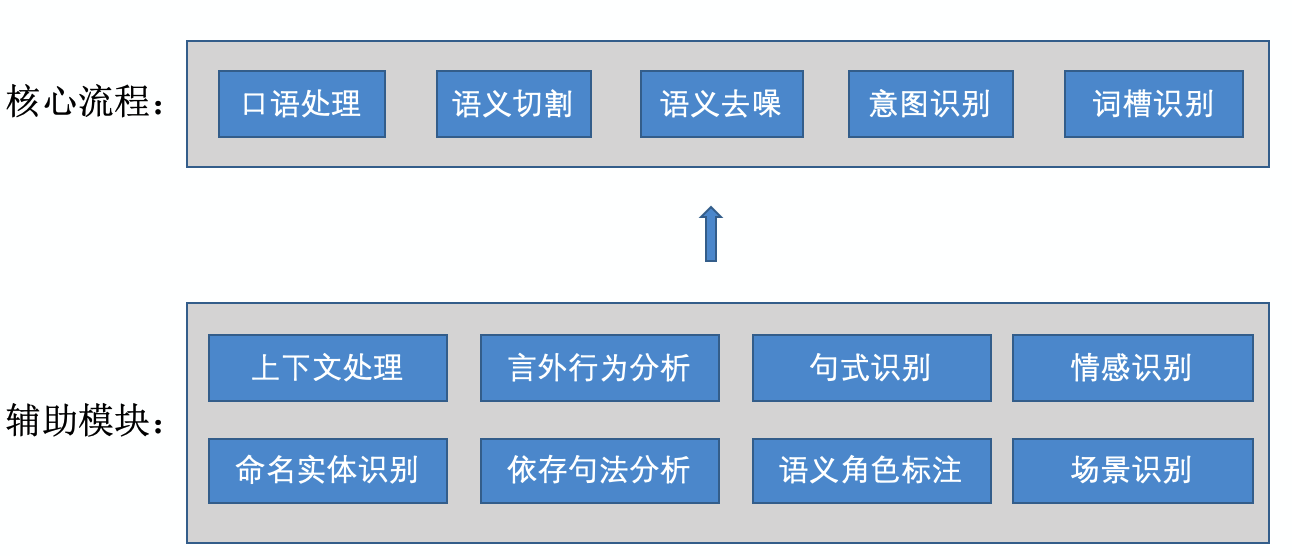
\includegraphics[scale=0.25]{chapters/nlu_process.png}
\caption{自然语言理解模块主要组成部分}
\label{fig:parserexample}
\end{figure}
然语言理解部分还有一些比较重要的模块比如句式识别,用户言外行为识别,上下文处理模块,场景识别模块,情感识别模块,依存语法分析模块和语义角色识别模块。其中句式识别主要用来识别是陈述句还是疑问句,疑问句会被优先输入意图识别模块,陈述句会被优先输入词槽抽取模块。用户言外行为识别可以用来识别用户是否在发出请求或者表达感谢,然后系统据此作出相应的回应。比如用户说”我要还款“,该句为陈述句,可能会被意图识别模块漏掉,但是一旦言外行为识别模型识别出这是用户请求,意图识别模块就会介入处理。

上下文处理模块在识别出当前问句语义成分不全的情况下用来改写当前问句得到完整的问句,然后再输入意图识别模块识别意图。场景识别模块用来识别当前聊天所处场景,用来辅助意图识别。情感识别可以有效的识别出用户当前的情绪,如果用户急躁或者抱怨的时候及时转人工处理以免影响用户体验。依存语法分析模块和语义角色识别模块会把用户问句转换成比较规范的中间语义表示格式,比如主谓宾,可以给包括意图识别在内的其他模块提供辅助。

对话状态跟踪模块~\cite{young2007hidden,henderson2014robust,henderson2014word},常见做法是把任务所需的所有槽位指定一个顺序,然后对每个槽位有一个状态变量标志着这个槽位是否已经被获取。另外一种做法是把对话状态定义为高维向量,然后联合训练口语理解模块和对话跟踪模块,使得联合模块直接预估对话状态。后者的好处是可以把两个模块进行联合训练,不需要人工设计规则。坏处是输出的高维向量人工难以解释,训练需要大量的标注数据,而且在标注数据缺乏的情况下不鲁棒。 

对话策略的实现方法分为基于规则的策略和基于强化学习~\cite{sutton1998reinforcement}的对话策略。一个最简单的基于规则的策略就是,对于对话状态中还未获取到的槽位,按顺序对用户进行提问,并且期望用户进行回答。
基于强化学习的对话策略把策略进行数学建模,策略以完成某种对话任务为目标,例如成功引导客人预订了酒店,或者成功销售某个商品。对话策略的目标由回报函数指定,如果策略成功引导对话状态完成了某种任务,那么这个策略会得到正的回报分数。常用对话策略是基于价值函数的强化学习框架中的Q-learning~\cite{watkins1989learning}。

自然语言生成模块有基于模板的方法和基于生成模型的方法。基于模板的回复生成方法,就是根据对话策略的输出选择合适的回复模板,然后把槽位值填在回复模板中的对应位置,这种方法不需要训练,实现简单。基于生成模型\cite{wen2015stochastic,wen2015semantically}的方法则会一个词接一个词地生成回复,直到生成完整句回复。大部分基于生成模型的方法都是基于递归神经网络RNN以及其变种,其特点在于比较灵活,不过需要大量的训练数据进行训练,而且生成的模型难以被人理解。

%\section{生成型对话系统}
% 定义
第三种对话系统,生成型对话系统\citep{sutskever2014sequence,shang2015neural,serban2016building,serban2016hierarchical},会根据用户的提问逐词地生成合适的回复。
% 好处
生成型系统最灵活,多用于对用户的问题进行闲聊式回复。
% 核心问题
% 常见方法
目前比较常见的方法是编码器解码器模型,还有很多新的方法使用了记忆模块,注意力模块等技术来改进生成型模型。
% 优点缺点总结
生成型对话很灵活,不过由于模型参数多,一般需要比较多的训练数据来进行训练。后面有一些使用预训练模型来减少模型所需训练数据的工作。除此之外,生成型对话系统容易产生不包含任何信息的``安全回复'',例如``我不知道''等。
%%%%%%%%%%%%%%%%%%%%% chapter.tex %%%%%%%%%%%%%%%%%%%%%%%%%%%%%%%%%
%
% sample chapter
%
% Use this file as a template for your own input.
%
%%%%%%%%%%%%%%%%%%%%%%%% Springer-Verlag %%%%%%%%%%%%%%%%%%%%%%%%%%
%\motto{Use the template \emph{chapter.tex} to style the various elements of your chapter content.}
\chapter{对话理解与智能质检}
\label{basic} % Always give a unique label
% use \chaptermark{}
% to alter or adjust the chapter heading in the running head
本节首先给出对话理解任务的定义,然后介绍对话理解的主要方法。接下来以智能质检为例,讲述对话理解是怎么落地和实现的。
\section{对话理解}
\subsection{什么是对话理解}
对话理解是指希望计算机跟人一样,具备自然语言理解的能力,从对话内容中挖掘对话意图,理解对话意图,用户情绪识别等。例如,在客服与用户交互的对话中,用户询问“今天的天气如何”,这里就是一个“询问天气”的意图。
这里对话可以包含语音对话和文本对话,如果是语音对话,我们一般可以利用语音自动识别技术将语音转为文本。后续我们要讨论的内容是文本的对话理解。
\subsection{技术路线分类}
一般而言,文本的对话理解从技术角度上可以分为两类:文本匹配和文本分类。

\textbf{文本匹配}~~~文本匹配的目标是得到$f(text_1, text_2)$的语义匹配得分,其中$text_1$和$text_2$是输入的文本,$f$是文本匹配模型。

\textbf{文本分类}~~~文本分类的目标则是得到${g(text)}$的类别标签,其中$text$是输入的文本,$g$是文本分类模型。在任务型对话中,类别标签就是意图。

\section{应用案例:智能质检}
对话理解在智能客服,智能质检有着广泛的应用。下面以智能质检为例,阐述对话理解相关技术是怎么应用的。
\subsection{什么是智能质检}

智能质检使用人工智能算法,分析坐席呼叫场景下人工客服与客户的对话,实现全量质量检查,提高人工客服的服务质量和客户的满意度。
智能质检系统的输入是一通人工客服和客户对话的录音,输出是质检报表,显示该录音在不同质检项的合格情况。质检项的重要性通过质检项的分数来决定。
智能质检无需人工介入,节省质检人力,覆盖率高(100\%),提升质检效率,降低漏检错检率。
\begin{figure}[h]
\centering
\includegraphics[scale=0.4]{./img/chapter4_b/qic_workflow.jpg}
\caption{智能质检基本流程图}
\label{fig1}
\end{figure}

从智能质检的基本流程图中我们可以发现,对话录音经过语音识别模块之后,我们得到了客户和人工客服之间的对话文本。质检员配置了质检项之后,我们将对话文本输入质检模型,最后得到了质检报表。
\subsection{实现方案与应用状况}
\textbf{实现方案}~~~假设我们定义了质检项要求客服在对话中“核实用户的工作地址”,比如“你的公司地址在哪里”。在冷启动时,一种简单的实现方案是通过规则配置“算子+逻辑操作符”或者正则表达式,如果录音文本中满足匹配条件,则命中该质检项。

如果我们有标注数据,就可以使用文本匹配和文本分类的方法。计算$f$(录音文本,质检例句)的语义匹配得分或者$g$(录音文本)的质检项标签。我们通过数据驱动的方法让模型越来越聪明,业务方只需要提供标注数据就能进行质检,不需要人工定义规则,模型具有一定的泛化能力。但遇到bad case没有基于规则的方法容易修复,另外需要标注数据积累到一定规模才能发挥模型的优势。

\textbf{应用状况}~~~当前智能质检的应用可以包含离线质检和坐席实时质检。离线质检是指结合语音识别和自然语言处理技术,对海量录音数据进行批量的智能化分析。离线质检在质检过程无需人工介入,可以提供内容质检,敏感词识别等质检结果。坐席实时质检是指在人工客服和客户通话过程中,提供实时质检功能,辅助人工客服判断客户情绪和实时分析对话过程的信息,及时提醒人工客服从而使客户获得更好的服务。现在智能质检的产品形态包含SaaS云服务和私有化部署。SaaS级产品部署,让中小企业也能够享受智能质检带来的高效与便捷,克服了采购费用高部署周期长的问题。

未来随着多方业务的使用,可以基于联邦学习进行智能质检,在满足数据安全和私隐保护的前提下,通过模型的参数梯度共享,获得了把所有数据放在一起训练的效果,使得不同的业务方合作共赢,建立更准确的数据模型。


\include{chapters/prospect}
%%%%%%%%%%%%%%%%%%%%% chapter.tex %%%%%%%%%%%%%%%%%%%%%%%%%%%%%%%%%
%
% sample chapter
%
% Use this file as a template for your own input.
%
%%%%%%%%%%%%%%%%%%%%%%%% Springer-Verlag %%%%%%%%%%%%%%%%%%%%%%%%%%
%\motto{Use the template \emph{chapter.tex} to style the various elements of your chapter content.}
\chapter{人脸识别}
\label{basic} % Always give a unique label
% use \chaptermark{}
% to alter or adjust the chapter heading in the running head


\section{问题定义}
人脸识别,是指对输入的图像和视频,检测其中存在的人脸,依据人脸的面部特征,完成身份识别的过程,属于生物特征识别技术。整个流程包含人脸检测、人脸对齐、人脸特征提取、人脸匹配几个阶段,如图 \ref{fig:face_recog_flow_chart} 所示。目前人脸识别已经广泛应用于安防、金融、军事等领域。

人脸识别具有以下优点:

自然性:所谓自然性,是指人脸识别技术所利用的生物特征,与人类进行人脸识别时所利用的生物特征是一致的,与之相比,虹膜识别、指纹识别等技术,则不具备自然性。

非接触性:在人脸识别技术中,用户不会与识别设备发生任何接触,对于用户来说体验较好。而指纹识别则需要用户进行按压设备。

使用便捷:用户使用人脸识别技术时非常方便,基本上无需做特殊的配合。

人脸识别也具有一些缺点,比如易受光照条件的影响,易受人脸遮挡物的影响,跨年龄识别难度较高等。但总的来说,人脸识别是目前一种可靠的,实用的,便捷的身份核验技术。

\begin{figure}[ht]
\centering
\includegraphics[scale=0.5]{img/chapter_fr/face_recog_flow_chart.png}
\caption{人脸识别流程图}
\label{fig:face_recog_flow_chart}
\end{figure}

\section{实现方案}
\subsection{人脸检测及对齐}
人脸检测是人脸识别的第一步,属于目标检测的子方向。其目的是找出图像中的人脸以及对应的位置。可能还会包含一些人脸的额外信息,比如人脸的关键点,姿态角度等。

典型的人脸检测是基于以下的流程:由于人脸可能出现的图像的任何位置,因此需要通过滑动窗口(sliding windows)来获取可能包含人脸的子图像。获取到的子图像,需要通过一个二分类的分类器,来判断图像中是否包含人脸,如果还需要确定人脸的精确位置,还需要加上一个回归人脸框的操作。同一个人脸可能会检测出多个人脸框,因此需要使用非极大值抑制(Non-Maximum suppression, NMS)来进行合并去重。接下来本文介绍一些具有代表性的人脸检测方法。

Viola-jones\cite{viola2001rapid}使用Haar-like小波特征,并通过级联的AdaBoost分类器构造检测器。该方法具有检测效率高,并且能够保持较好的精度的特点,是第一个具有实用意义的人脸检测算法。MTCNN\cite{zhang2016joint}将人脸分类、人脸框回归以及人脸关键点定位在同一个任务内完成了,是一个多任务(multi-task)的检测方法,这种思路在后续的很多方法里也得到了使用。

anchor的思想在目标检测方法Faster-rcnn\cite{ren2015faster}中首先被提出,在人脸检测中也经常使用到。anchor提出的目的是为了解决目标在图像中可能以不同的形状存在,比如不同的长宽比,所以加入人工的先验信息,预先定义不同比例的anchor来进行候选目标框的获取。Face r-cnn\cite{wang2017face}, Pyramidbox\cite{tang2018pyramidbox}, Retinaface\cite{deng2019retinaface}这些方法,都用到了anchor的思想。另一个在人脸检测中经常使用的思想是特征金字塔网络(feature pyramid network),为了自适应不同尺度人脸的检测,一般有两种做法,一种做法是图像金字塔,这种方法需要对输入图像做不同尺度的缩放,缺点是耗时较高;另一种更好的做法则是特征金字塔,其思想是在不同分辨率的特征图(feature map)上检测对应尺度的目标,同时将不同分辨率的特征图与更高层的特征图进行特征融合,保证每一层的特征图都具有足够的表达能力。Pyramidbox,Retinaface都用到了特征金字塔,SSH\cite{najibi2017ssh}虽然没有直接用到特征金字塔,但其也是对网络3个不同尺度的特征图进行分别预测,来解决多尺度的人脸检测问题。

做完人脸检测后,一般需要进行人脸对齐。通过对人脸进行关键点定位,以及预先定义好的关键点模板,进行仿射变换,通过旋转、平移、缩放等操作,进行人脸对齐,对齐后的人脸能够更好的进行人脸特征提取。目前常见的关键点个数,有5个关键点、68个关键点、90个关键点以及106个关键点等。

\subsection{人脸特征提取}
特征提取是人脸识别的关键步骤,它将人脸图像映射都某个特征空间中,使得映射后的特征能够很好地区分不同人之间的差异点。经过特征提取得到人脸的特征表示之后,可以进行特征匹配。如果是对两个特征进行比对,我们一般称为人脸比对或者人脸验证(verification),如果是将一个特征与一组特征进行匹配,我们一般称为人脸检索或者人脸识别(identification),如图 \ref{fig:verification_identification} 所示。

\begin{figure}[ht]
\centering
\includegraphics[scale=0.55]{img/chapter_fr/verification_identification.png}
\caption{人脸特征抽取}
\label{fig:verification_identification}
\end{figure}

传统的特征提取算法,通过一些降维方法,得到一系列降维后的特征,用来表示人脸。比如使用PCA进行降维的EigenFace,基于LDA进行降维的FisherFace等,都是早期人脸识别中非常经典的算法。但这些方法存在一些缺点,对光照、表情、姿态敏感,泛化能力不足,因此在实际使用中的准确度不高。

随着深度学习的广泛应用,越来越多具有实用价值的方法被提出,人脸识别的研究得到了极大的发展。基于深度学习的特征提取方法可以分为两大类:
\paragraph{度量学习(metric learning)}
通过一个度量函数,来衡量相同人或者不同人的特征表示之间的距离,从而学习到每个人每个照片的特征表示,基本思路是同一个人的特征表示之间的距离尽可能小,不同人的特征表示的距离尽可能大。
这一个方向的典型方法包含2014年的Contrastive loss\cite{sun2014deep}和2015年google提出的Triplet loss\cite{schroff2015facenet}。

DeepID2是基于Contrastive loss的模型,它在训练的时候,同时训练classification和verification两个信号,其中的verification信号,就是用特征表示之间的Contrastive loss来构造的。Contrastive loss是基于pairwise的思想,模型训练时,需要输入两张图片,如果两个图片是同一个人,则verification的标签为1,如果不是同一个人,则标签为0。

google于2015年提出的Facenet中,则用到了Triplet loss。其思想是以三元组的形式来训练模型,每次输入需要三张图片,其中两张图片是同一个人,以及一张其他人的图片,要求同一个人的照片之间的距离要小于不同人之间的距离,且要超过一个margin。

\paragraph{基于margin的分类方法(margin based classification)}
第二类思想是基于分类的思想来进行特征提取,根据训练集中的数据,同一个人的照片属于同一类,训练集一共包含多少个id,则总共需要分多少类。由于用的分类的思想,所以自然而然可以使用分类的损失函数。而在此基础上,又提出了一系列的方法,用以最小化类内间距或者最大化类间间距。比较有代表性的方法有Center loss\cite{wen2016discriminative},SphereFace\cite{liu2017sphereface},CosFace\cite{wang2018cosface}以及ArcFace\cite{deng2019arcface}等。

由于是多分类任务,所以最基本的损失函数形式是softmax loss。但是直接用softmax loss训练出来的特征,往往效果不理想,某些类别的类内间距甚至比类间间距大,导致人脸识别的时候出现错误。Center loss引入了类内中心,为每个类别提供一个类内中心,最小化训练集中每个样本与其类内中心的距离,从而达到减少类内间距的效果。

基于SphereFace的训练方式,是在此基础上做了改进,对权重进行了归一化,且增加了角度裕量,在cos函数上对角度乘上因子m,加大分类难度。CosFace和ArcFace更进一步,对特征表示也做了归一化,并分别引入了不同的margin形式,取得了更好的效果。

以上方法都是通过不同方式去减少同一个人的类内间距以及增大不同人之间的类间间距。但除了损失函数以及网络的设计之外,更为重要的是训练的数据的分布,比较好的训练数据是同一个人包含多张不同的照片,这些照片覆盖此人不同年龄段,不同姿态角度,不同遮挡程度,不同妆容情况等,这样的数据能够学习到鲁棒性更强,通用性更好的模型。
\section{应用案例}

人脸识别目前在安防、金融等领域都得到了广泛应用,下面介绍一些常见的应用案例。
\paragraph{门禁闸机}
这是人脸识别的典型应用场景,属于人脸检索(1:N)的应用。门禁闸机在初始化的时候,会要求录入一个人脸库,该人脸库经过特征提取后,作为识别的底库。当有人通过闸机的时候,会拍摄来人的照片,通过特征提取转化为特征表示之后,与底库中的特征集合进行对比,找出该人员是否存在于底库中。
\paragraph{金融核身业务}
目前几乎所有的金融核身业务都支持人脸核身功能,属于人脸比对(1:1)的应用。当用户的办理某些业务的时候,会被要求进行人脸核身,系统会通过摄像头采集用户的照片,与用户留底的另一张照片进行比对,以确定用户是否为本人。这种方式大大减少了金融业务中进行业务审核的人员数量及审核时间,节省了用户时间,提升了用户体验。

\include{chapters/voiceprint}
\include{chapters/other_bio_recog}
\include{chapters/anti_spoofing}
\bibliographystyle{gbt7714-2005}
\bibliography{chapters/reference}

\backmatter%%%%%%%%%%%%%%%%%%%%%%%%%%%%%%%%%%%%%%%%%%%%%%%%%%%%%%%
%\include{glossary}
%\include{solutions}
\printindex

%%%%%%%%%%%%%%%%%%%%%%%%%%%%%%%%%%%%%%%%%%%%%%%%%%%%%%%%%%%%%%%%%%%%%%

\end{document}





